\documentclass[journal,12pt,twocolumn]{IEEEtran}
\usepackage{setspace}
\usepackage{gensymb}
\usepackage{caption}
%\usepackage{multirow}
%\usepackage{multicolumn}
%\usepackage{subcaption}
%\doublespacing
\singlespacing
\usepackage{csvsimple}
\usepackage{amsmath}
\usepackage{multicol}
%\usepackage{enumerate}
\usepackage{amssymb}
%\usepackage{graphicx}
\usepackage{newfloat}
%\usepackage{syntax}
\usepackage{listings}
\usepackage{iithtlc}
\usepackage{color}
\usepackage{tikz}
\usetikzlibrary{shapes,arrows}



%\usepackage{graphicx}
%\usepackage{amssymb}
%\usepackage{relsize}
%\usepackage[cmex10]{amsmath}
%\usepackage{mathtools}
%\usepackage{amsthm}
%\interdisplaylinepenalty=2500
%\savesymbol{iint}
%\usepackage{txfonts}
%\restoresymbol{TXF}{iint}
%\usepackage{wasysym}
\usepackage{amsthm}
\usepackage{mathrsfs}
\usepackage{txfonts}
\usepackage{stfloats}
\usepackage{cite}
\usepackage{cases}
\usepackage{mathtools}
\usepackage{caption}
\usepackage{enumerate}	
\usepackage{enumitem}
\usepackage{amsmath}
%\usepackage{xtab}
\usepackage{longtable}
\usepackage{multirow}
%\usepackage{algorithm}
%\usepackage{algpseudocode}
\usepackage{enumitem}
\usepackage{mathtools}
\usepackage{hyperref}
%\usepackage[framemethod=tikz]{mdframed}
\usepackage{listings}
    %\usepackage[latin1]{inputenc}                                 %%
    \usepackage{color}                                            %%
    \usepackage{array}                                            %%
    \usepackage{longtable}                                        %%
    \usepackage{calc}                                             %%
    \usepackage{multirow}                                         %%
    \usepackage{hhline}                                           %%
    \usepackage{ifthen}                                           %%
  %optionally (for landscape tables embedded in another document): %%
    \usepackage{lscape}     


\usepackage{url}
\def\UrlBreaks{\do\/\do-}


%\usepackage{stmaryrd}


%\usepackage{wasysym}
%\newcounter{MYtempeqncnt}
\DeclareMathOperator*{\Res}{Res}
%\renewcommand{\baselinestretch}{2}
\renewcommand\thesection{\arabic{section}}
\renewcommand\thesubsection{\thesection.\arabic{subsection}}
\renewcommand\thesubsubsection{\thesubsection.\arabic{subsubsection}}

\renewcommand\thesectiondis{\arabic{section}}
\renewcommand\thesubsectiondis{\thesectiondis.\arabic{subsection}}
\renewcommand\thesubsubsectiondis{\thesubsectiondis.\arabic{subsubsection}}

% correct bad hyphenation here
\hyphenation{op-tical net-works semi-conduc-tor}

%\lstset{
%language=C,
%frame=single, 
%breaklines=true
%}

%\lstset{
	%%basicstyle=\small\ttfamily\bfseries,
	%%numberstyle=\small\ttfamily,
	%language=Octave,
	%backgroundcolor=\color{white},
	%%frame=single,
	%%keywordstyle=\bfseries,
	%%breaklines=true,
	%%showstringspaces=false,
	%%xleftmargin=-10mm,
	%%aboveskip=-1mm,
	%%belowskip=0mm
%}

%\surroundwithmdframed[width=\columnwidth]{lstlisting}
\def\inputGnumericTable{}                                 %%
\lstset{
%language=C,
frame=single, 
breaklines=true,
columns=fullflexible
}
 

\begin{document}
%
\tikzstyle{block} = [rectangle, draw,
    text width=3em, text centered, minimum height=3em]
\tikzstyle{sum} = [draw, circle, node distance=3cm]
\tikzstyle{input} = [coordinate]
\tikzstyle{output} = [coordinate]
\tikzstyle{pinstyle} = [pin edge={to-,thin,black}]

\theoremstyle{definition}
\newtheorem{theorem}{Theorem}[section]
\newtheorem{problem}{Problem}
\newtheorem{proposition}{Proposition}[section]
\newtheorem{lemma}{Lemma}[section]
\newtheorem{corollary}[theorem]{Corollary}
\newtheorem{example}{Example}[section]
\newtheorem{definition}{Definition}[section]
%\newtheorem{algorithm}{Algorithm}[section]
%\newtheorem{cor}{Corollary}
\newcommand{\BEQA}{\begin{eqnarray}}
\newcommand{\EEQA}{\end{eqnarray}}
\newcommand{\define}{\stackrel{\triangle}{=}}

\bibliographystyle{IEEEtran}
%\bibliographystyle{ieeetr}

\providecommand{\nCr}[2]{\,^{#1}C_{#2}} % nCr
\providecommand{\nPr}[2]{\,^{#1}P_{#2}} % nPr
\providecommand{\mbf}{\mathbf}
\providecommand{\pr}[1]{\ensuremath{\Pr\left(#1\right)}}
\providecommand{\qfunc}[1]{\ensuremath{Q\left(#1\right)}}
\providecommand{\sbrak}[1]{\ensuremath{{}\left[#1\right]}}
\providecommand{\lsbrak}[1]{\ensuremath{{}\left[#1\right.}}
\providecommand{\rsbrak}[1]{\ensuremath{{}\left.#1\right]}}
\providecommand{\brak}[1]{\ensuremath{\left(#1\right)}}
\providecommand{\lbrak}[1]{\ensuremath{\left(#1\right.}}
\providecommand{\rbrak}[1]{\ensuremath{\left.#1\right)}}
\providecommand{\cbrak}[1]{\ensuremath{\left\{#1\right\}}}
\providecommand{\lcbrak}[1]{\ensuremath{\left\{#1\right.}}
\providecommand{\rcbrak}[1]{\ensuremath{\left.#1\right\}}}
\theoremstyle{remark}
\newtheorem{rem}{Remark}
\newcommand{\sgn}{\mathop{\mathrm{sgn}}}
\providecommand{\abs}[1]{\left\vert#1\right\vert}
\providecommand{\res}[1]{\Res\displaylimits_{#1}} 
\providecommand{\norm}[1]{\left\Vert#1\right\Vert}
\providecommand{\mtx}[1]{\mathbf{#1}}
\providecommand{\mean}[1]{E\left[ #1 \right]}
\providecommand{\fourier}{\overset{\mathcal{F}}{ \rightleftharpoons}}
%\providecommand{\hilbert}{\overset{\mathcal{H}}{ \rightleftharpoons}}
\providecommand{\system}{\overset{\mathcal{H}}{ \longleftrightarrow}}
	%\newcommand{\solution}[2]{\textbf{Solution:}{#1}}
\newcommand{\solution}{\noindent \textbf{Solution: }}
\newcommand{\myvec}[1]{\ensuremath{\begin{pmatrix}#1\end{pmatrix}}}
\providecommand{\dec}[2]{\ensuremath{\overset{#1}{\underset{#2}{\gtrless}}}}
\DeclarePairedDelimiter{\ceil}{\lceil}{\rceil}
%\numberwithin{equation}{section}
%\numberwithin{problem}{subsection}
%\numberwithin{definition}{subsection}
\makeatletter
\@addtoreset{figure}{section}
\makeatother

\let\StandardTheFigure\thefigure
%\renewcommand{\thefigure}{\theproblem.\arabic{figure}}
\renewcommand{\thefigure}{\thesection}


%\numberwithin{figure}{subsection}

%\numberwithin{equation}{subsection}
%\numberwithin{equation}{section}
%\numberwithin{equation}{problem}
%\numberwithin{problem}{subsection}
\numberwithin{problem}{section}
%%\numberwithin{definition}{subsection}
%\makeatletter
%\@addtoreset{figure}{problem}
%\makeatother
\makeatletter
\@addtoreset{table}{section}
\makeatother

\let\StandardTheFigure\thefigure
\let\StandardTheTable\thetable
\let\vec\mathbf
\numberwithin{equation}{section}

\vspace{3cm}


\title{%Convex Optimization in Python
	\logo{
	Random Numbers
	}
}
%\title{
%	\logo{Matrix Analysis through Octave}{\begin{center}\includegraphics[scale=.24]{tlc}\end{center}}{}{HAMDSP}
%}


% paper title
% can use linebreaks \\ within to get better formatting as desired
%\title{Matrix Analysis through Octave}
%
%
% author names and IEEE memberships
% note positions of commas and nonbreaking spaces ( ~ ) LaTeX will not break
% a structure at a ~ so this keeps an author's name from being broken across
% two lines.
% use \thanks{} to gain access to the first footnote area
% a separate \thanks must be used for each paragraph as LaTeX2e's \thanks
% was not built to handle multiple paragraphs
%

\author{Rishit D$^{*}$% <-this % stops a space
}% <-this % stops a space
%\thanks{J. Doe and J. Doe are with Anonymous University.}% <-this % stops a space
%\thanks{Manuscript received April 19, 2005; revised January 11, 2007.}}
}
% note the % following the last \IEEEmembership and also \thanks - 
% these prevent an unwanted space from occurring between the last author name
% and the end of the author line. i.e., if you had this:
% 
% \author{....lastname \thanks{...} \thanks{...} }
%                     ^------------^------------^----Do not want these spaces!
%
% a space would be appended to the last name and could cause every name on that
% line to be shifted left slightly. This is one of those "LaTeX things". For
% instance, "\textbf{A} \textbf{B}" will typeset as "A B" not "AB". To get
% "AB" then you have to do: "\textbf{A}\textbf{B}"
% \thanks is no different in this regard, so shield the last } of each \thanks
% that ends a line with a % and do not let a space in before the next \thanks.
% Spaces after \IEEEmembership other than the last one are OK (and needed) as
% you are supposed to have spaces between the names. For what it is worth,
% this is a minor point as most people would not even notice if the said evil
% space somehow managed to creep in.



% The paper headers
%\markboth{Journal of \LaTeX\ Class Files,~Vol.~6, No.~1, January~2007}%
%{Shell \MakeLowercase{\textit{et al.}}: Bare Demo of IEEEtran.cls for Journals}
% The only time the second header will appear is for the odd numbered pages
% after the title page when using the twoside option.
% 
% *** Note that you probably will NOT want to include the author's ***
% *** name in the headers of peer review papers.                   ***
% You can use \ifCLASSOPTIONpeerreview for conditional compilation here if
% you desire.




% If you want to put a publisher's ID mark on the page you can do it like
% this:
%\IEEEpubid{0000--0000/00\$00.00~\copyright~2007 IEEE}
% Remember, if you use this you must call \IEEEpubidadjcol in the second
% column for its text to clear the IEEEpubid mark.



% make the title area
\maketitle

\tableofcontents

\bigskip

\renewcommand{\thefigure}{\theenumi}
\renewcommand{\thetable}{\theenumi}

\begin{abstract}
Solutions to Random Numbers
\end{abstract}
%%

\section{Uniform Random Numbers}
Let $U$ be a uniform random variable between 0 and 1.
\begin{enumerate}[label=\thesection.\arabic*
,ref=\thesection.\theenumi]
\item Generate $10^6$ samples of $U$ using a C program and save into a file called uni.dat .
\\
\solution Download the following files. 
\begin{lstlisting}
wget https://github.com/gadepall/probability/raw/master/manual/codes/exrand.c
wget https://github.com/gadepall/probability/raw/master/manual/codes/coeffs.h
\end{lstlisting}

Now execute the following code.
\begin{lstlisting}
gcc exrand.c -lm
./a.out
\end{lstlisting}

%
\item
Load the uni.dat file into python and plot the empirical CDF of $U$ using the samples in uni.dat. The CDF is defined as
\begin{align}
F_{U}(x) = \pr{U \le x}
\end{align}
\\
\solution  The following code plots Fig. \ref{fig:uni_cdf}
\begin{lstlisting}
wget https://github.com/gadepall/probability/raw/master/manual/codes/cdf_plot.py
python3 cdf_plot.py
\end{lstlisting}
\begin{figure}[!ht]
\centering
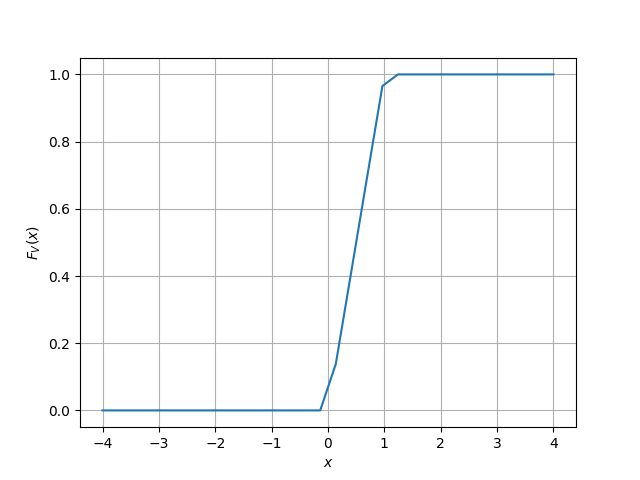
\includegraphics[width=\columnwidth]{../figs/uni_cdf.png}
\caption{The CDF of $U$}
\label{fig:uni_cdf}
\end{figure}

%
\item
Find a theoretical expression for $F_{U}(x)$.
\\
\solution Given $U$ is a uniformly distributed random variable over the interval $(0, 1)$, we have the density function $p_U(x)$:

	\begin{align}
		p_U(x) = 
		\begin{cases}
			1, & x \in (0, 1) \\
			0, & otherwise
		\end{cases}
		\label{eq:PDF}
	\end{align}
	
	We know

	\begin{align}
		F_U(x) = \int_{-\infty}^{x} p_U(x) \,dx
		\label{eq:Relation}
	\end{align}
	
	Given $U$ is a uniformly distributed random variable over the interval $(0, 1)$, we have the following expression for $F_U(x)$:
	
	\begin{align}
		F_U(x) = 
		\begin{cases}
			0, & x \in (-\infty, 0) \\
      			x, & x \in (0, 1) \\
      			1, & x \in (1, \infty)
    		\end{cases}
	\end{align}

\item
The mean of $U$ is defined as
%
\begin{equation}
E\sbrak{U} = \frac{1}{N}\sum_{i=1}^{N}U_i
\end{equation}
%
and its variance as
%
\begin{equation}
\text{var}\sbrak{U} = E\sbrak{U- E\sbrak{U}}^2 
\end{equation}

Write a C program to  find the mean and variance of $U$.
\\
\solution
\\
Execute the following commands on linux terminal:
\begin{lstlisting}
gcc mean_var_uni.c -lm
./a.out
\end{lstlisting}

\item Verify your result theoretically given that
\end{enumerate}
%
\begin{align}
E\sbrak{U^k} = \int_{-\infty}^{\infty}x^kdF_{U}(x)
\end{align}
\\
\solution
This can be alternatively wriiten as
	\begin{align}
		E[U^k] = \int^{\infty}_{-\infty} x^k p_U(x) \,dx
		\label{eq: Expected}
	\end{align}

We know that mean $\mu$ is given by $E(U)$. Hence
	\begin{align}
		\mu = \int_{-\infty}^{\infty} x p_U(x) \,dx
		\label{eq:Relation_1}
	\end{align}

	\begin{align}
		\mu &= \int_{0}^{1} x \,dx \\
		&= \frac{x^2}{2} \Bigg|^{1}_{0} \\
		&= \fbox{$\frac{1}{2}$} 
		\label{eq: Mean}
	\end{align}
	
We know
	\begin{align}
		var(U) = E((U - E(U))^2)
	\end{align}

	This can also be represented as
	\begin{align}
		var(U) &= E(U^2 - 2E(U)U + (E(U))^2) \\
		&= E(U^2) - 2(E(U))^2 + (E(U))^2 \\
		&= E(U^2) - (E(U))^2
		\label{eq: Relation_2}
	\end{align}

We can evaluate $E(U^2)$ using \eqref{eq: Expected} as:
	\begin{align}
		E(U^2) &= \int_{-\infty}^{\infty} x^2 p_U(x) \,dx \\
		&= \int_{0}^{1} x^2 \,dx \\
		&= \frac{x^3}{3} \Bigg|^{1}_{0} \\
		&= \frac{1}{3}
	\end{align}

Using \eqref{eq: Mean} and \eqref{eq: Relation_2} we have
	\begin{align}
		var(U) = \frac{1}{3} - \frac{1}{4} = \fbox{$\frac{1}{12}$}
	\end{align}

Using this, we obtain mean as $0.5007$ and variance as $0.083301$. Hence the statistically obtained values are in close agreement with the theoretical values of $\mu = 0.5$ and $\sigma^2 = \frac{1}{12}$.


\section{Central Limit Theorem}
%
\begin{enumerate}[label=\thesection.\arabic*
,ref=\thesection.\theenumi]

%
\item
Generate $10^6$ samples of the random variable
%
\begin{equation}
X = \sum_{i=1}^{12}U_i -6
\end{equation}
%
using a C program, where $U_i, i = 1,2,\dots, 12$ are  a set of independent uniform random variables between 0 and 1
and save in a file called gau.dat.
\\
\solution
To generate samples for the Gaussian distribution, run the following code
\begin{lstlisting}
gcc exrand.c -lm
./a.out
\end{lstlisting}

%
\item
Load gau.dat in python and plot the empirical CDF of $X$ using the samples in gau.dat. What properties does a CDF have?
\\
\solution The CDF of $X$ is plotted in Fig. \ref{fig:gauss_cdf}
\begin{figure}
\centering
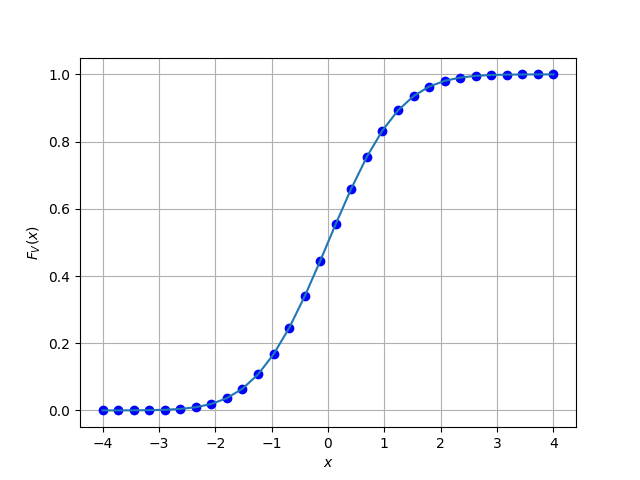
\includegraphics[width=\columnwidth]{../figs/gau_cdf.png}
\caption{The CDF of $X$}
\label{fig:gauss_cdf}
\end{figure}


\item
Load gau.dat in python and plot the empirical PDF of $X$ using the samples in gau.dat. The PDF of $X$ is defined as
\begin{align}
p_{X}(x) = \frac{d}{dx}F_{X}(x)
\end{align}
What properties does the PDF have?
\\
\solution The PDF of $X$ is plotted in Fig. \ref{fig:gauss_pdf} using the code below
\begin{lstlisting}
wget https://github.com/gadepall/probability/raw/master/manual/codes/pdf_plot.py
python3 pdf_plot.py
\end{lstlisting}

\begin{figure}
\centering
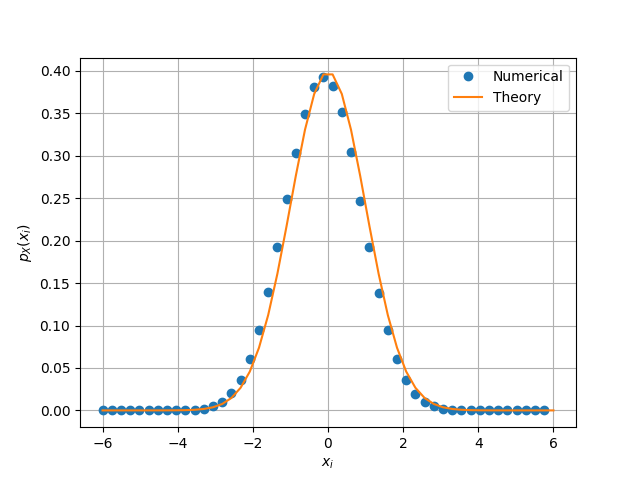
\includegraphics[width=\columnwidth]{../figs/gauss_pdf.png}
\caption{The PDF of $X$}
\label{fig:gauss_pdf}
\end{figure}

\item Find the mean and variance of $X$ by writing a C program.
\\
\solution
\\
The mean and variance is given by the following code:
\begin{lstlisting}
gcc mean_var_gau.c -lm
./a.out
\end{lstlisting}

\item Given that 
\begin{align}
p_{X}(x) = \frac{1}{\sqrt{2\pi}}\exp\brak{-\frac{x^2}{2}}, -\infty < x < \infty,
	\label{eq:PDF_2}
\end{align}
repeat the above exercise theoretically.
\\
\solution Given
	\begin{align}
		F_X(x) = \int_{-\infty}^{x} p_X(x) \,dx
		\label{eq:Relation_3}
	\end{align}

	We have, using 
	\eqref{eq:Relation_3} and 
	\eqref{eq:PDF_2}
	\begin{align}
		F_X(x) = \int_{-\infty}^{x} \frac{1}{\sqrt{2\pi}}\exp{\frac{-x^2}{2}} \,dx
	\end{align}
	
	Mean for random variable $X$ is given by:
	
	\begin{align}
		\mu_x &= E(X) \\
		&= \int^{\infty}_{-\infty} x p_X(x) \,dx \\
		&= \int^{\infty}_{-\infty} \frac{x}{\sqrt{2\pi}}\exp{\left(\frac{-x^2}{2}\right)} \,dx \\
		&= \fbox{0}
	\end{align}

	Note that the integral
	\begin{align}
		\int^a_{-a} f(x) \,dx
	\end{align}
	becomes 0, when $f(x)$ is odd.
	
	Variance for random variable $X$ is given by:

	\begin{align}
		var(X) = E(X^2) - (E(X))^2
		\label{eq: MeanVar}
	\end{align}

	We evaluate $E(X^2)$ as follows:

	\begin{align}
		E(X^2) &= \int^{\infty}_{-\infty} x^2 p_X(x) \,dx \\
	\end{align}

	Using integration by parts, we have:
	\begin{align}
		E(X^2) &= -x\sqrt{\frac{2}{\pi}} e^{\left(\frac{-x^2}{2}\right)}\Bigg|_{-\infty}^{\infty} +  \int^{\infty}_{-\infty} \sqrt{\frac{2}{\pi}} e^{\left(\frac{-x^2}{2}\right)} \,dx \\
		&= 1
		\label{eq: MeanSec}
	\end{align}

	Hence using \eqref{eq: MeanVar} and \eqref{eq: MeanSec}, we have

	\begin{align}
		var(X) &= E(X^2) - (E(X))^2 \\
		&= 1 - 0^2 \\
		&= \fbox{1}
	\end{align}
Using this, we obtain the statistical mean and variance to be 0.000326 and 1.000906 respectively which is in close agreement with the theoretical values.

	%
\end{enumerate}
\section{From Uniform to Other}
\begin{enumerate}[label=\thesection.\arabic*
,ref=\thesection.\theenumi]
%
\item
Generate samples of 
%
\begin{equation}
V = -2\ln\brak{1-U}
\end{equation}
%
and plot its CDF.
\\
\solution
The following can be used to generate samples for random variable $V$:
\begin{lstlisting}
gcc new_v.c -lm
.\a.out
\end{lstlisting}

The following code can be used to generate CDF for $V$:
\begin{lstlisting}
python3 log_cdf.py
\end{lstlisting}
The figure generated is shown as \eqref{fig:log_cdf}

\begin{figure}
\centering
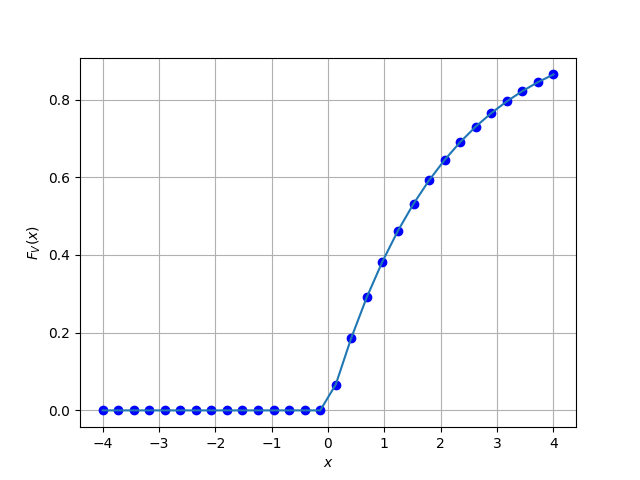
\includegraphics[width=\columnwidth]{../figs/log_cdf.png}
\caption{The PDF of $V$}
\label{fig:log_cdf}
\end{figure}
  
\item Find a theoretical expression for $F_V(x)$.
\\
\solution
We have been given that random variable $V$ is a function of the random variable $U$ as follows:
	
	\begin{align}
		V = -2\ln{(1 - U)}
		\label{eq:FuncRV}
	\end{align}

	Note that the obtained distribution function (CDF) for random variable $U$ is:

	\begin{align}
		F_U(x) = 
		\begin{cases}
			0, & x \in (-\infty, 0) \\
			x, & x \in (0, 1) \\
			1, & x \in (1, \infty)
		\end{cases}
		\label{eq:CDF_U}
	\end{align}

We know for any random variable $X$

	\begin{align}
		F_X(x) = \Pr(X \leq x)
		\label{eq:CDF_Def}
	\end{align}

	Hence, we can write using \eqref{eq:FuncRV} and \eqref{eq:CDF_Def}

	\begin{align}
		F_V(x) &= \Pr(V \leq x) \\
		&= \Pr(-2\ln{(1 - U)} \leq x)\\
		&= \Pr(\ln{(1 - U)} \geq \frac{-x}{2})\\
		&= \Pr(1 - U \geq \exp{\frac{-x}{2}})\\
		&= \Pr(U \leq 1 - \exp{\frac{-x}{2}})\\
		&= F_U(1 - \exp{\frac{-x}{2}})
		\label{eq: CDF_Rel}
	\end{align}

Note that the function $f(x) = 1 - \exp{\left(\frac{-x}{2}\right)}$ follows:
	\begin{align}
		f(x) \in
		\begin{cases}
			{0}, & x \in (-\infty, 0) \\
			(0, 1) & x \in (0, \infty)
		\end{cases}
	\end{align}

	Hence we can write
	\begin{align}
		F_V(x) = 
		\begin{cases}
			0, & x \in (-\infty, 0) \\
			1 - \exp{\left(\frac{-x}{2}\right)}, & x \in (0, \infty)
    		\end{cases}
	\end{align}

%
%\item
%Generate the Rayleigh distribution from Uniform. Verify your result through graphical plots.
\end{enumerate}


\end{document}


